% !TEX program = xelatex
\documentclass[a4paper]{article}
\usepackage{amsmath}
\usepackage{amsthm}
\usepackage[left=1.8cm,right=1.8cm,top=2.2cm,bottom=2.0cm]{geometry}
\usepackage{ctex}
\usepackage{enumerate}
\usepackage{fancyhdr}
\usepackage{xpatch}
\usepackage{graphicx} 
\usepackage{float} 
\usepackage{subfigure} 
\usepackage{amsfonts}
\usepackage{mathtools}
\usepackage{framed}
\usepackage{multicol}
\usepackage{listings}
\usepackage{hyperref}
\usepackage{tikz}
\usetikzlibrary{automata,positioning}
\theoremstyle{definition}
\newtheorem*{solution*}{\textbf{Solution:}}
\newtheorem*{proof*}{\textbf{Proof:}}
\newtheorem{theorem}{Theorem}[subsection]
\newtheorem{definition}{Definition}[subsection]
\newtheorem{lemma}{Lemma}[subsection]
\makeatletter
\usepackage{listings}% http://ctan.org/pkg/listings
\lstset{
  basicstyle=\ttfamily\tiny,
  mathescape,
}
\AtBeginDocument{\xpatchcmd{\@thm}{\thm@headpunct{.}}{\thm@headpunct{}}{}{}}
\makeatother

\pagestyle{fancy}
\renewcommand{\baselinestretch}{1.15}

\usepackage{paralist}
\let\itemize\compactitem
\let\enditemize\endcompactitem
\let\enumerate\compactenum
\let\endenumerate\endcompactenum
\let\description\compactdesc
\let\enddescription\endcompactdesc

% shorten footnote rule
\xpatchcmd\footnoterule
  {.4\columnwidth}
  {1in}
  {}{\fail}

\title{CS 131 Compilers: Discussion 10: A software egineers' view over compilation behaviour}
\author{\textbf{杨易为}~~\textbf{季杨彪}~~\textbf{尤存翰} \\ \texttt{ \{yangyw,jiyb,youch\}@shanghaitech.edu.cn}}


\begin{document}
\maketitle
\section{Scope}
From today on, we steps into a new topic: semantic. We cast analysis on the grammar from CFG and do as many checks as possible, during which we mark something like type, scope and runtime garbage collector so that they can do better in runtime.
\subsection{Dynamic Scoping}
A global identifier refers to the identifier associated with the most recent environment, and is uncommon in modern languages. In technical terms, this means that each identifier has a global stack of bindings and the occurrence of a identifier is searched in the most recent binding.

\begin{lstlisting}[language=C]
// Since dynamic scoping is very uncommon in 
// the familiar languages, we consider the 
// following pseudo code as our example. It
// prints 20 in a language that uses dynamic
// scoping.   
  
int x = 10;
  
// Called by g()
int f()
{
   return x;
}
  
// g() has its own variable
// named as x and calls f()
int g()
{
   int x = 20;
   return f();
}
  
main()
{
  printf(g());
}
\end{lstlisting}
\subsection{Lexical Scoping}

\textbf{Scoping} refers to the issue of matching \href{https://docs.python.org/zh-cn/3.9/reference/compound_stmts.html#class-definitions}{identifier declarations} with its Uses. The \textbf{Scope} of an identifier is the portion of a program where it is accessible.
\begin{enumerate}
  \item Same identifier may refer to different things in different portions.
  \item Different scopes for same identifier \textbf{Do Not} overlap.
  \item Usually, search for \textbf{local} definition first, and if not found, goto its parent Scope.
\end{enumerate} 

\subsubsection{Python Scoping}
\
In python, we have 4 kinds of scopes and their life cycle.

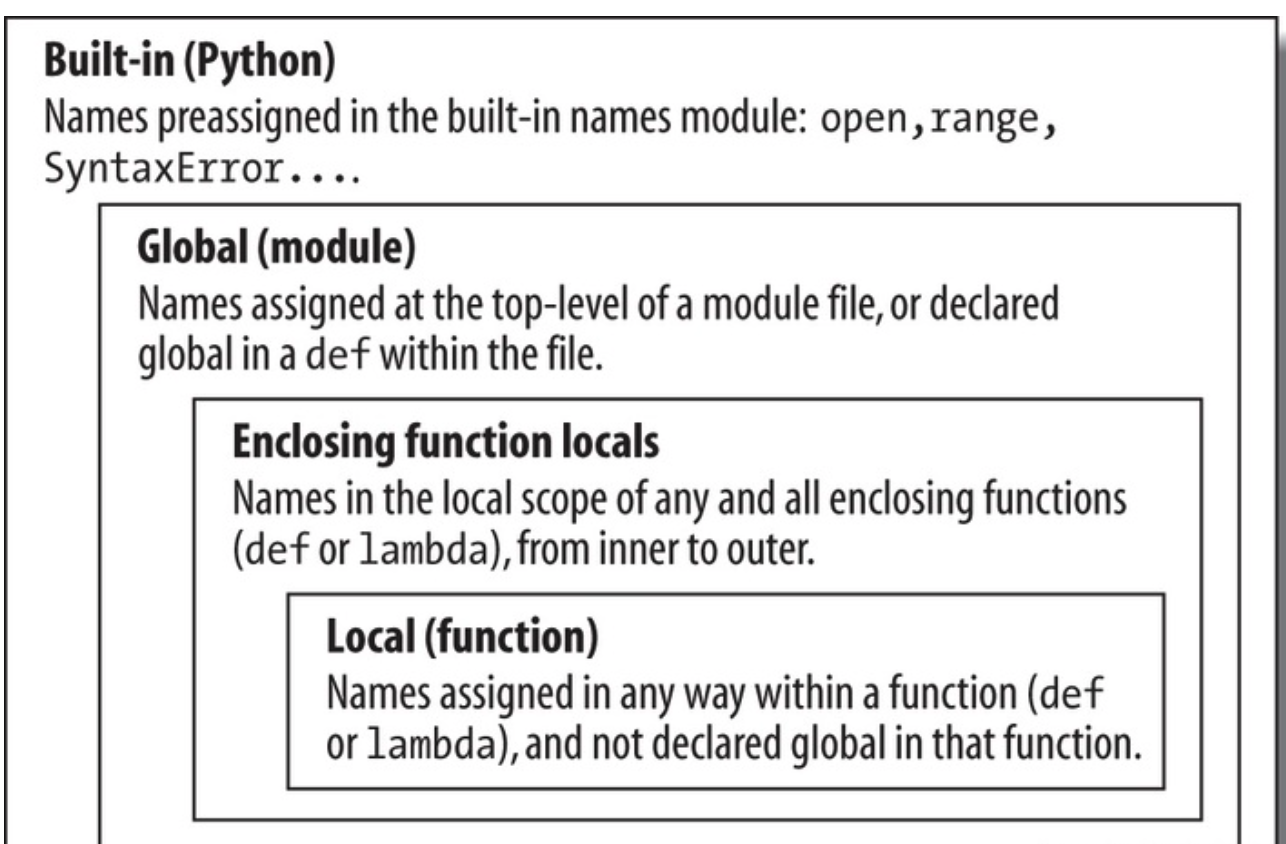
\includegraphics[width=14cm]{img/Snipaste_2021-04-24_02-41-32.png}
\begin{enumerate}
  \item local scope,  that is, the temporary variables defined in the function, when the function ends, the life cycle of the variable ends.

  \item enclosed (closure, the local scope of the nested parent function), that is, the local variables of the outer function of the closure, the end of the outer function, the end of the life cycle of the variable.
  \item global (global variables), that is, variables defined at the module level, the module is destroyed, the life cycle of the variable will end.
  \item bulit-in (built-in function) is the python interpreter, the virtual machine built-in variables.
\end{enumerate}

Here we put a benign testcases and adversarial testcases
\begin{enumerate}
  \item 
  \begin{lstlisting}

  \end{lstlisting}
  \item \begin{lstlisting}
def f(): # runtime error
    a = 123
    def g():
        exec "print a"
    g()

def f(): # compile error
    a = 123
    def g():
        exec "print a"
        print a
    g()

def f(): # runtime error
    a = 123
    def g():
        print eval("a")
    g()

def f(): # print 123
    a = 123
    def g():
        print eval("a")
        print a
    g()
  \end{lstlisting}
\end{enumerate}
\begin{lstlisting}
struct LetList {
  vector<pair<Expr, Expr>> l;
  Expr plug(const Expr & e) const {
    Expr ret(e);
    for (auto it = l.rbegin(); it != l.rend(); ++it) {
      ret = Let(it->first, it->second, ret);
    }
    return ret;
  }
  Expr let(const Expr & val) {
    Expr id(Var());
    l.push_back(pair<Expr, Expr>(id, val));
    return id;
  }
  function<Expr()> llet(const Expr & val) {
    return [this, val](){ return let(val); };  // notice that this is a pointer, so the return is invalidated when LetList die.
  }
  static Expr with(const function<Expr(LetList &)> & f) {
    LetList ll;
    return ll.plug(f(ll));
  }
};

// A ScopedLet is a list of letlist that support scoping instead of mindlessly append at front.
struct ScopedLet {
  vector<LetList> ll;
  struct Frame {
    ScopedLet & sl;
    Frame(ScopedLet & sl) : sl(sl) {
      sl.ll.push_back(LetList());
    }
    ~Frame() {
      assert(sl.ll.size() != 0, "cannot be empty");
      sl.ll.pop_back();
    }
    LetList * operator->() {
      assert(sl.ll.size() != 0, "cannot be empty");
      return & sl.ll.back();
    }
  };
  Expr with(const function <Expr(Frame &)> & f) {
    Frame fr(self);
    return fr->plug(f(fr));
  }
};
\end{lstlisting}
\section{Type System}
Type is very important to 
\end{document}
